\chapter{Debugging in Robotics}

%[Write about the difficulties in robot debugging in general as a short introduction]

% excerpt from icra paper
Traditional debugging tools mostly rely on breakpoints, a mechanism to interrupt the execution of a program at a specific place in the program code. This can be a problem for robotic applications since they usually can not be interrupted in their execution, because the robots generally don't run in a deterministic and suspendable environment \cite{Gumbley2009}. Interrupting a robotic application would destroy the continuity in which the sensors collect data, the environment of the robot would change substantially and thus the robot's behaviour would change, which is an example of the ``probe effect'' and makes it hard to reproduce a fault unless it has a single cause \cite{Gumbley2009}. This makes it necessary to collect data during debugging without interrupting the execution of the program.

%[write about text only problem here]
Another problem with traditional debugging tools is that they usually render data collected during debugging as text and it's the developer's task to interpret the data. In a suspendable environment the developer has as much time as they need to interpret and analyse the data. When debugging robotic applications the developer usually has a lot less time, because of the uninterruptible nature of the application. The data in robotic applications is usually too complex to understand in its raw representation, for example quaternions to specify 3D positions. In order to help the developer understand the data faster, graphical tools have been developed to support the developer. Due to many different application scenarios in robotics and the diverse environment of available frameworks for robot development, many researchers and developers have built their own tools to support them during debugging \cite{Collett2010}. This has lead to a high amount of different debugging tools for different purposes.

This chapter gives an overview of tools and practices currently in use to debug robotic applications. The first section covers some instrumented tools which do not require source code modifications, instead they rely on more technical solutions. The second section summarizes logging mechanisms which are also often used for debugging. Although not all of the logging mechanisms presented in section two are related to robotic systems they represent a class of debugging tools which are often used in robotics. The tools presented in the first two sections mainly focus on debugging without interrupting the execution of a robotic application. Section three introduces graphical systems that aim to support the developer during the debugging task. The last section focuses on tools for the development with ROS. Section three and four both present tools which have been developed to bridge the gap between the robots' perception of the world and the developer's understanding of the collected data.

%Imagine a robot is developed which is supposed to follow people through the house.  It is impossible to interrupt the execution of the robot to debug a specific problem, because the environment in which the robot is tested will change while the robot is interrupted and thus not sensing anything. The situation in which the robot should be debugged changes 

%%%% INSTRUMENTED TOOLS %%%%
\section{Instrumented Debugging Tools}
This section introduces some of the most instrumented  debugging tools used for robotics. The tools presented in this section usually don't require source code modification, they use special operating system hooks to control the execution of an application and collect data during the runtime. These kind of tools are usually external tools and are not associated with a robotics framework or middleware, they can be used independent of the framework or middleware.

\subsection{GDB}
%[overview, general introduction to gdb]
The GNU Project Debugger (GDB) is a general purpose debugger, originally designed to debug C and C++ programs, but other languages have been added later on. The debugger ``allows you to see what is going on `inside' another program while it executes'' \cite{Stallman2002}. GDB is open source and free software, released under the GNU General Public License (GPL). Although GDB is a highly sophisticated tool with many features, this section will summarize only the features that are most important for robotics. A more detailed overview of GDB's features can be found on the project website\footnote{http://www.gnu.org/software/gdb/} and in the book ``Debugging with GDB: The GNU Source-Level Debugger'' \cite{Stallman2002}.

The emerging market of embedded systems and robotics triggered the development of new features like the support for debugging remote targets and collecting data with tracepoints instead of breakpoints. These features are particularly important for robotics, since robotic applications are in general not interruptible and often mobile, which means the source code is executed on a different machine from where it is developed.

\subsubsection{Remote Debugging}
Some times it is impossible or infeasible to run GDB on the target platform itself. In robotics this might be due to limited processing power on the target machine or due to a special operating system on the target machine which does not support debugging. GDB can connect to remote targets running on different machines, if the program on the remote machine has been executed with \verb+gdbserver+. \verb+gdbserver+ is an auxiliary program which implements a debugging stub. The debugging stub contains a set of subroutines which take care of the communication with the GDB host through a GDB specific remote serial protocol \cite{Stallman2002}. Once the remote target is connected to the host, it can be controlled remotely: the developer can use GDB to specify breakpoints and control the execution of the program.

The debugging stub is specific to the architecture of the remote target. GDB distributes a couple of already implemented debugging stubs for certain architectures, but if another target platform is used the stub needs to be implemented.

\subsubsection{GDB Tracepoints}
%[introduce gdb tracepoints and their downside (postmortem analysis)]
As already mentioned, in some occasions it can be impractical to interrupt a program during its execution. Especially in robotics it is important to have a way to collect data during debugging without interrupting the execution of the program. GDB's \verb+trace+ and \verb+collect+ commands can be used to specify locations in the program code where data should be collected \cite{Stallman2002}. These locations are called tracepoints and are similar to breakpoints: they mark a location in the source code which is important to the developer. The data can be collected with arbitrary expressions which are evaluated when a tracepoint is hit, without interrupting the execution.

The collected data can be analysed after the program has stopped its execution. The collected data is stored in a buffer on the remote target and represents snapshots of the data values that have been specified when the tracepoint was created. Each snapshot can be analysed closely using the normal GDB commands (e.g. \verb+backtrace+ and \verb+print+) as if the target would still be running \cite{Stallman2002}.

GDB tracepoints are currently only available for remote targets. If you want to collect data with tracepoints in a local program, it has to be started with \verb+gdbserver+ and handled like a remote target.

\subsection{Realtime Debugging Tracepoints}
%[Luke Gumbleys work, tracepoint theory, adaptation in robotics, instrumentation]
The tracepoints approach presented above has one major downside: data can only be accessed and analysed after the program has stopped. This might be necessary for some systems, where transmitting the data over the network is too much overhead and can cause the system to fail. On the other hand there are systems that take a long time to properly start up and shut down. In such systems the GDB tracepoints approach will make development cumbersome and slow.

To counter this problem, a realtime debugging framework for robotics was developed \cite{Gumbley2009}. It uses GDB to collect data when a tracepoint is hit, but transmits the data immediately to the user interface. The data can be accessed live during a debugging session and the developer does not need to wait for the application to stop to evaluate the data.

A plugin for the NetBeans IDE\footnote{http://netbeans.org/} integrated the novel debugging tool to make it easier to use. The user interface to set traditional breakpoints was re-used for tracepoints and presents a well known interface for developers. The user interface can be extended with further plugins to visualize the data collected during debugging. The first plugins created for this tool rendered laser and ultrasonic rangefinder data \cite{Gumbley2009}.

%[significant configuration overhead]

%[modules need to be compiled with debugging symbols]


%%%% LOGGING FRAMEWORKS %%%%
\section{Logging Frameworks}

The previous section presented tools to collect data without the need to modify the source code. This section presents tools from the other end of the spectrum: Using logging and print statements is a popular method to collect data during debugging. Although logging frameworks originally were developed for long term collection of data, they can also be used excessively during the development of a particular feature or module. Logging statements help developers to understand the flow of execution in a program and can be used flexibly to output data values during the execution of the program.

[double check]: 
This section presents logging facilities from various robotic frameworks and summarizes where the differences are and what points they have in common.


\subsection{Logging in ROS}
\label{ros_logging}

\subsection{Logging in Player/Stage}

\subsection{Logging in Orca}

\subsection{Print Statements}
Although print statements are not part of a "logging framework", they are often used in the same way as other logging statements. Print statements are quite popular amongst developers because no additional knowledge is required to use them and they are a core part of every major programming language and thus don't require to link external libraries. Print messages are simpler then logging statements, they print a String message to a console and have no feature to filter or visualize the printed data.

The use of print statements is a really flexible way of collecting data during debugging. The major downside of print statements is that it is easy to loose the overview where print statements have been used. If they are not excluded from the build before the software is released, this can lead to a weaker performance of the software.

The text only representation of messages printed on the console restricts the use of print statements to the most basic types of data, since more complex data would be too hard to understand in its raw representation. This is especially true in robotics, since the data in robotics usually comes from sensors and complex algorithms. Despite the text only limitation, developers can pre select what they want to print and can use the full power of the programming language they are using to aggregate values or compute simple metrics and properties for complex data which might be useful during debugging.

%[point out that it is flexible but can become a problem in bigger projects because the logging statements for debugging are often forgotten and not removed. managing where such statements are in the code can be a problem.]

%[probably unrelated to debugging in robotics? maybe have a section "other debugging tools?" or summarize this in the ROS logging as other logging frameworks]
%\subsection{Android LogCat}
%\subsection{Java Log4j}

%%%% GRAPHICAL DEBUGGING AIDS %%%%
\section{Graphical Debugging Systems}
This section gives an overview of the graphical tools to support debugging in robotics. Those graphical tools are often used to get a better understanding of the robots position in the real world and to visualize sensor readings and control values. Visualization is an important factor in robotics, because developers usually cannot interrupt the execution of a robot and take as much time as they need to understand data. They need to get as much information out of the data stream as possible in a very short time to detect problems and their causes.

\subsection{LabVIEW}

LabVIEW (Laboratory Virtual Instrumentation Engineering Workbench) is a graphical programming environment developed by National Instruments\footnote{http://www.ni.com}. It features \emph{Front Panels} which allow a developer to add widgets to a graphical interface. These widgets can display the status of the graphical program or act as control interface (button, knobs, etc.) for the program. For each widget on a panel an element is created in the block diagram of the program which can be connected to other parts in the block diagram. LabVIEW delivers a high number of pre-defined visualization widgets such as text displays, sliders and progress bars, which can be used to create a dedicated user interface for an application. This user interface can be used to control the application as well as monitor and debug the application. Fig.~\ref{labview_screenshot} shows the LabVIEW user interface with a front panel in the background.

% source: public domain image from http://en.wikipedia.org/wiki/File:WikipediaFPandBD.png
\begin{figure}[htbp]
  \centering
  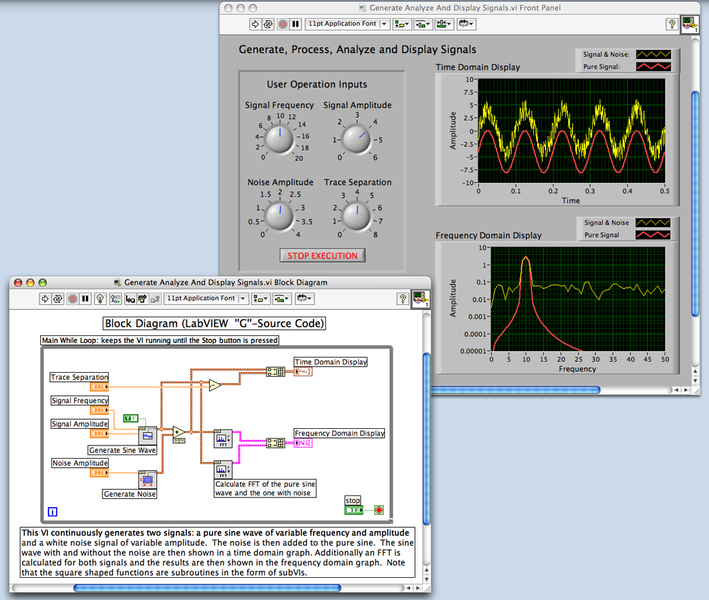
\includegraphics[scale=0.45]{img/labview_frontpanel.png}
  \caption{Screenshot of the LabVIEW user interface with front panels in the top right.}
  \label{labview_screenshot}
\end{figure}

The front panel feature was described as ``LabVIEW's biggest advantage,'' its ``best feature,'' or its ``main power'' in the open-format answers of a survey of LabVIEW programmers \cite{Whitley2001}. It would be possible to design concrete front panels also for the purpose of debugging a specific application. This however requires integrating each front panel element directly into the visual program and is thus highly intrusive. Though a more transparent debugging possibility would be desirable, LabVIEW shows the potential of a flexible tool for visualization of abstract data in form of graphical widgets.

\subsection{Augmented Reality Debugging System}
ARDev is an augmented reality (AR) debugging system based on Player/Stage \cite{Collett2010}. The AR approach to debugging helps the developer to understand the global state of the robot by augmenting a video feed of the robot with information of the robots' perception. Like the tools presented above, it focuses on pre-defined data such as laser and sonar sensors. The visualization of abstract data has been identified as possible future work \cite{Collett2010}. Initial evaluation studies were promising that the visualization can help developers significantly during debugging \cite{Collett2010}.

\subsection{Microsoft Robotics Studio}
\cite{Jackson2007} ---> I'll probably drop this. MS robotics studio has not much relevance for my work...

%%%% DEBUGGING IN ROS %%%%
\section{Visual Debugging in ROS}
\label{debugging_ros}

%[summarize what ros is]
ROS (Robot Operating System) \cite{Quigley2009} is an Open Source framework for complex robotic systems which has grown significantly in the last years, has an active community backing the project and supports many of the currently available robots \cite{Foote2012}. It was developed to abstract from the hardware of the robot and make it easier to create modular robot software, which can run on different robots and on different machines. The modular approach makes development easier, because the work can be divided amongst different developers or development teams. This also allows the developer to change only small parts of a complex system, without the need to build and re-deploy the whole system.
The modules in ROS are called \emph{nodes} and several nodes executed together are called a \emph{stack}. ROS \emph{packages} bundle nodes and stacks and are used to make software modules available to other developers. Everyone can create their own package which can be indexed by ROS so that their software modules can be found, downloaded and used by other developers. There exist many packages, nodes and stacks with implementations of algorithms for some of the most common problems in robotics (e.g. navigation, localization, joint movement, etc.) and they can easily be (re-)used.

The communication between ROS nodes is either asynchronous through a publish/subscribe mechanism or synchronous through services. Nodes can send messages by publishing a message on a topic and receive messages by subscribing to that topic. This mechanism is flexible and decouples the sender from the receiver. A publisher node does not need to know if there are other nodes listening and vice versa. For synchronous communication and guaranteed delivery of messages, services can be invoked. The routing is established during runtime through the ROS core. The communication between nodes is one of the main sources for debugging data when debugging a ROS application. The same communication framework is also used for the logging mechanism in ROS, which publishes messages to the special purpose topic \emph{/rosout}.

This section gives an overview of the ROS tools that can be used to monitor the ROS communication channels and thus debug ROS applications. ROS has both command line tools and tools with a graphical interface. Often there is a graphical interface based on the command line tool, in which case this section will focus on the graphical part, since it basically has the same functionality as the command line interface.

%[skip next paragraph]
%ROS comes with several tools to assist the developers during the development and debugging of a robot. The tools most relevant to this work are:
%\begin{description}[\setlabelwidth{rxconsole}]
%\item[rostopic] a command line tool to monitor topics and publish messages on topics.
%\item[rxplot] a graphical tool which plots data from one or more topic fields on a cartesian coordinate system.
%\item[rxconsole] displays logging messages that have been published on the special purpose topic \emph{/rosout}.
%\item[rviz] renders models of the robot in 3D and visualizes spatial data like point clouds, robot poses, trajectories, etc. \cite{Quigley2009}.
%\end{description}

\subsection{RViz}
\label{rviz}
[maybe I should move RViz to graphical debugging tools and rename this section to "other debugging tools in ROS" or drop? rxbag can be moved to the graphical section as well and the rest is pretty basic (not sure what to do with rxplot, but rxconsole can be merged with ROS logging)]

Most of the currently available robot frameworks have their own tools for data visualization, this section presents RViz as representative for the class of visualization tools in robotics. Other visualization tools with similar features are playerv from the Player/stage framework \cite{Gerkey2003}, OrcaView2d and OrcaView3d from ORCA \cite{Makarenko2006} and robotgui from CARMEN \cite{Montemerlo2003} which is a more general user interface.

RViz\footnote{http://www.ros.org/wiki/rviz} is a highly sophisticated graphical interface to render 3-dimensional data. The tool visualizes a 3d model of the robot (Figure~\ref{rviz_model}) and can visualize additional data like point clouds (Figure~\ref{rviz_pcl}), maps, robot poses, trajectories, etc. \cite{Quigley2009}. During the development of robot applications, it is hard to understand how the robot perceives his surroundings, because the robot is bound by sensor data which might not always collect information accurately enough. This leads to problems during the execution which are hard to identify, reproduce and investigate due to the indeterministic nature of robotic applications. RViz helps developers to understand how the robot sees the world and makes it easier to understand what caused a problem.

% source: CC image from http://www.ros.org/wiki/rviz/DisplayTypes/RobotModel
\begin{figure}[htbp]
  \centering
  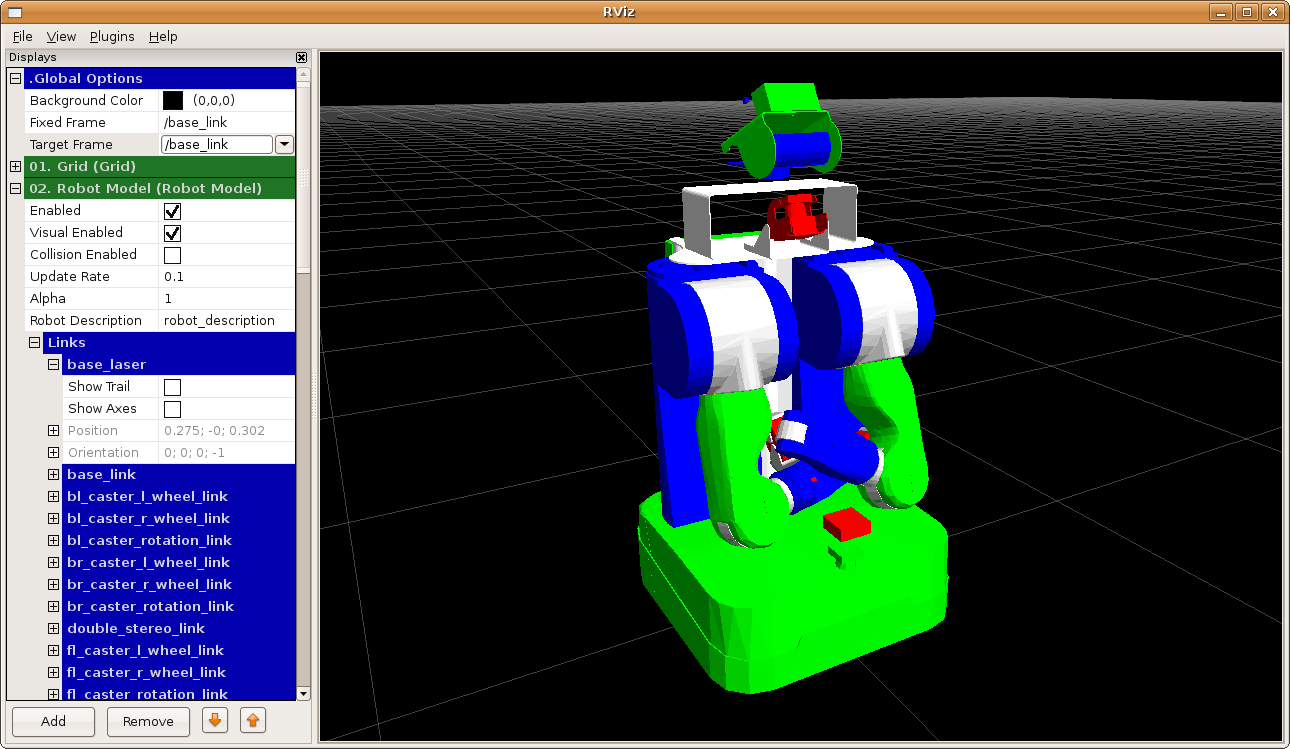
\includegraphics[scale=0.3]{img/RVizRobotModel.png}
  \caption{3D model of a PR2 robot in RViz. Source: \url{http://www.ros.org/wiki/rviz/DisplayTypes/RobotModel}, License: Creative Commons Attribution 3.0}
  \label{rviz_model}
\end{figure}

% source: CC image from http://www.ros.org/wiki/rviz/DisplayTypes/RobotModel
\begin{figure}[htbp]
  \centering
  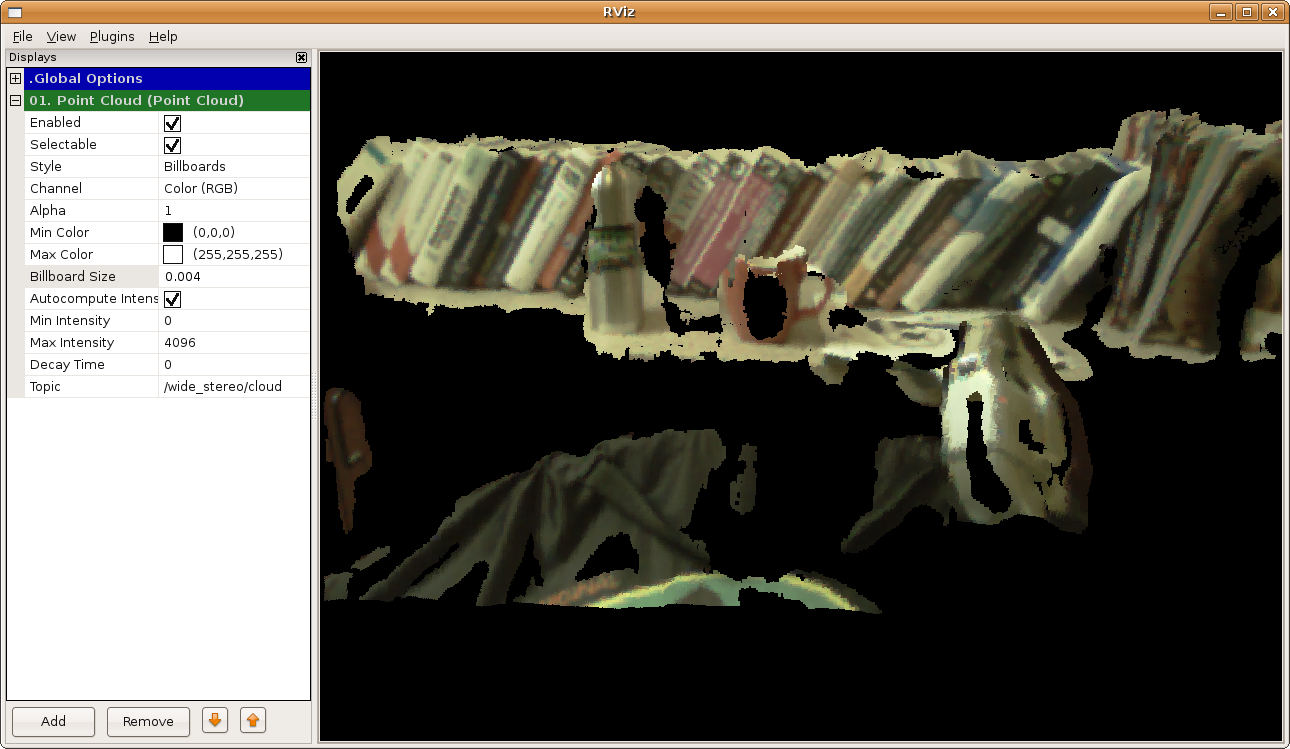
\includegraphics[scale=0.3]{img/RVizPointCloud.png}
  \caption{Point cloud visualization in RViz.\\Source: \url{http://www.ros.org/wiki/rviz/DisplayTypes/PointCloud}, License: Creative Commons Attribution 3.0}
  \label{rviz_pcl}
\end{figure}

%\begin{figure}[htbp]
%  \centering
%	\begin{minipage}{\textwidth}%
%		\subfigure[3D model of a PR2 robot in RViz. Source: \url{http://www.ros.org/wiki/rviz/DisplayTypes/RobotModel}, License: Creative Commons Attribution 3.0]{
%				%\rule{4cm}{3cm}
%				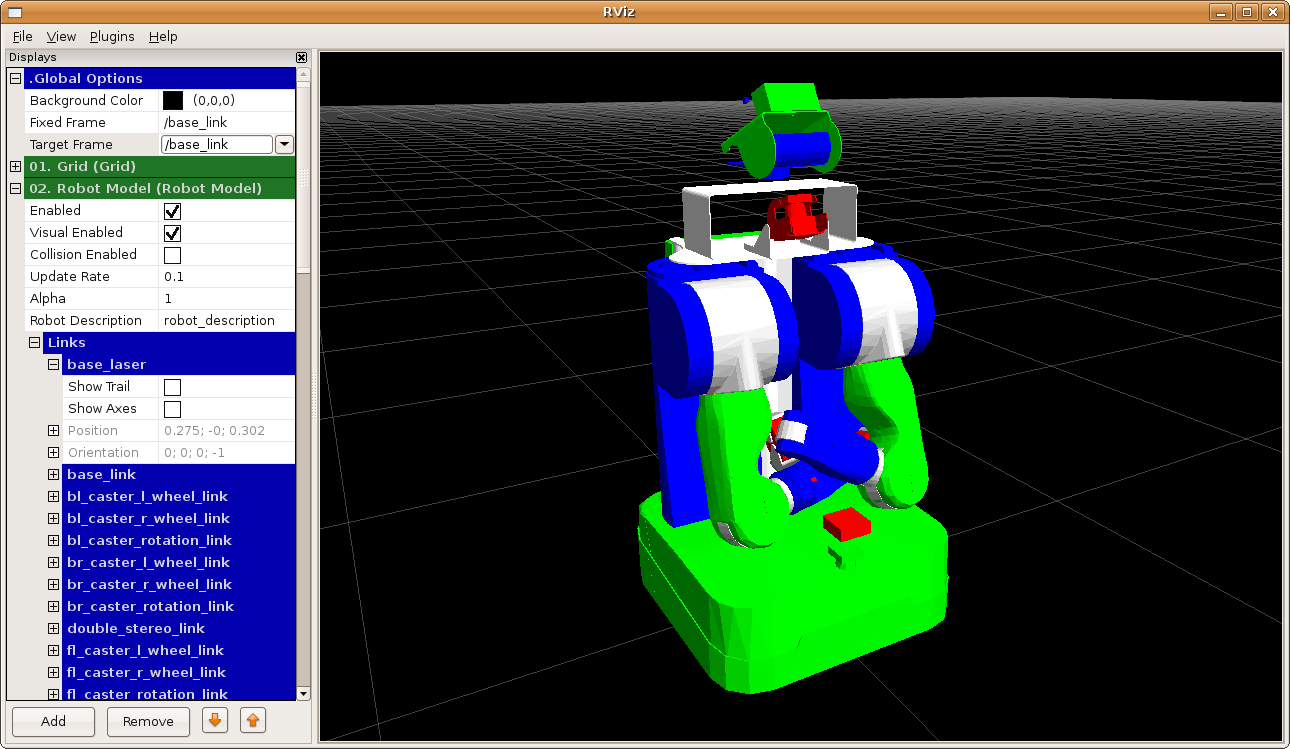
\includegraphics[scale=0.1]{img/RVizRobotModel.png}
%				\label{rviz_model}
%		}

%		\subfigure[Point cloud visualization in RViz. Source: http://www.ros.org/wiki/rviz/DisplayTypes/PointCloud, License: Creative Commons Attribution 3.0]{
%				%\rule{4cm}{3cm}
%				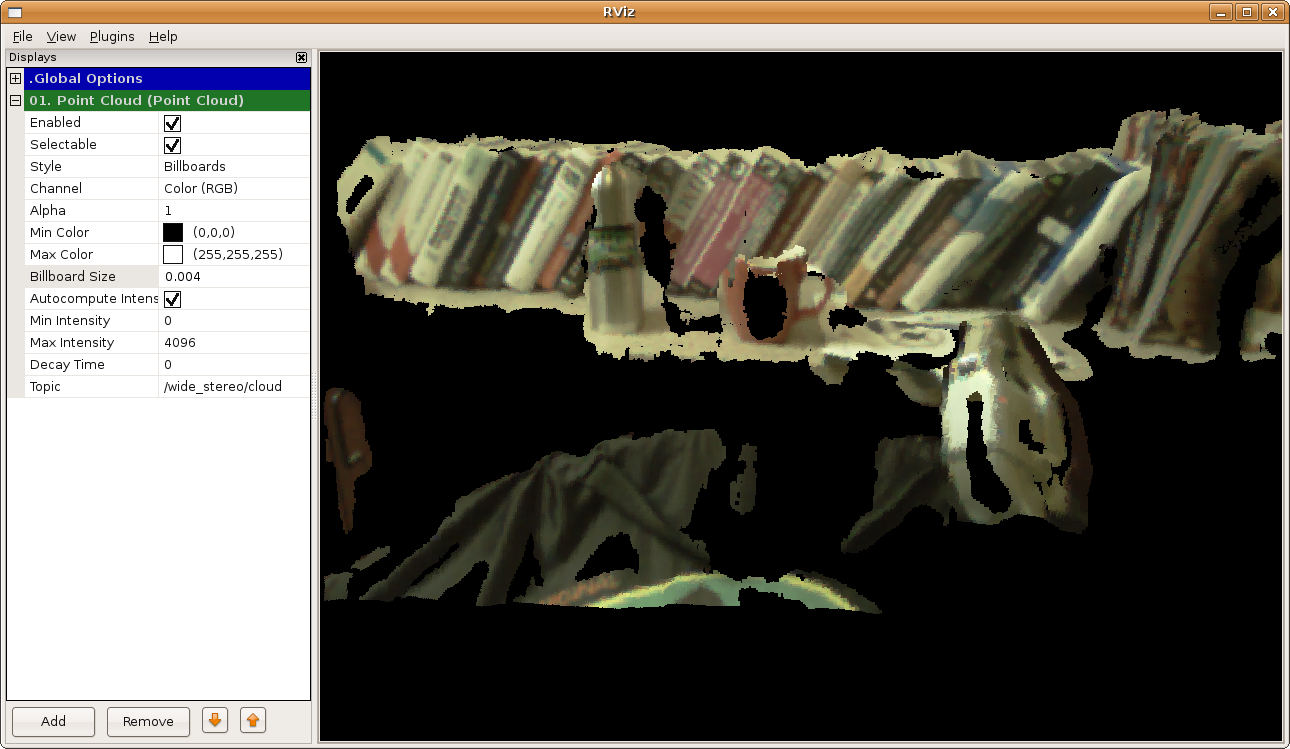
\includegraphics[scale=0.1]{img/RVizPointCloud.png}
%				\label{rviz_pcl}
%		}
%	\end{minipage}%

%	\caption{Screenshots of different visualization types in RViz.}
%\end{figure}

RViz requires a 3d model with the exact proportions of the robot to visualize the robot and its movement correctly. The data visualized in RViz is mostly pre-defined and collected from known interfaces such as laser sensors, mapping algorithms and computer vision modules. Although it is possible to visualize arbitrary data in RViz, it is hard to find a good place to visualize the data, because the data does not have to be directly related to the real world, it can also be intermediate values from a computation algorithm.

The plugin funcionality in RViz can be used to extend RViz with further visualizations and modules. The current plugin interface is not not documented yet, since it is under active development and the plugin API is expected to change significantly before it will be released with the next major ROS release \cite{rvizPlugin}.

\subsection{rxconsole}
rxconsole is a graphical user interface to display messages that have been published on the special purpose topic \emph{/rosout}. The special purpose topic \emph{/rosout} is used by the ROS logging framework (see \ref{ros_logging}). rxconsole keeps a list of messages with additional information like the severity of the message, the node which published the message and the timestamp when the message was published. The tool also allows filtering by severity and text.

[screenshot?]

rxconsole is designed to only display text messages since the logging framework converts everything to a text message before publishing. Important information about the type of data is not preserved. rxconsole is thus a very simple tool to monitor logging messages, it does not offer any special visualization for data, which would be hard since the messages are text based and don't contain type information.

\subsection{rxbag}
In a complex robotic system there is usually a lot of communication happening at once. Trying to keep track of the different topics and messages is not an easy task and recording the messages for analysis at a later stage is necessary. rosbag is a tool to dump communication data from selected topics to a file for later use or to analyse the communication after the application has terminated. The data is stored in a so called bag-file, which contains all the messages published to selected topics during the runtime of the application. rosbag can also be used to play back the recorded messages in the same order and with the same time offset as they were recorded. This can be used to examine the behaviour of one particular subsystem without the need of running the full stack of subsystems in a real environment.

[example use of rosbag?]

The bag-file can also be used to examine a flow of events in the system after the execution has terminated. rxbag is a graphical tool to analyse bag-files, it visualizes the content of a bag-file on a timeline. The tool has controls to play back, pause and rewind the stream of messages, which allows to have a closer look at some events on the timeline. rxbag visualizes image messages as thumbnails on the timeline which makes it easier to understand what the robot was facing when the messages were recorded. Developers can use rxbag to inspect messages in more detail, since the raw messages were recorded and can be accessed from the tool.

[rxbag screenshot?]

While rxbag mostly focuses on replaying recorded messages from a bag file, it can also be used to visualize the data stream while it records it. This can be done with the command line option \emph{--record}. rxbag can be extended with more visualizations through a plugin API. The plugin API is still experimental and under development, but it should become more stable in future versions of ROS \cite{rxbag}.

[epiphany: difference between rosdashboard and rxbag: rxbag focuses on recorded data, but can also do live visualization. The biggest difference is that rxbag needs a static configuration (what topics should be recorded) and does not allow ad-hoc addition of new topics which might only be used for debugging reasons. This makes the configuration more time consuming because after adding a new logging statement the whole capturing process needs to be adapted and restarted to get the new data. rosdashboard can be left untouched, only a new widget needs to be added]

%rxbag does something similiar we do: visualize data. It visualizes data from a bag file: you can see image data in a picture-stream way, plot numerical data and look at raw messages. You can also write plugins for more visualizations. The downside is that it only operates on pre-collected data sets (bags) and not on live data. This would be interesting to explore further, to visualize data live and collect the data for later analysis (combining rxbag with rosdashboard). This would not be a big problem, because collecting the bag file while we are visualizing is not a problem.

\subsection{rxplot}
rxplot is a graphical tool which can plot values from topics on a Cartesian coordinate system. 

\subsection{RQT - ROS GUI}
--> remove, not related to debugging. can be introduced in rosdashboard when reasons for the choice of ros are presented (rosdashboard integrates well with other tools in the ros environment and recently many graphical tools were developed)
\subsection{rxDeveloper}
[\textbf{outline, results of the survey, importance for this work}]
\cite{Muellers2012}

[Not really debugging, this might go somewhere else? Maybe not a full subsecion but only a couple of sentences that summarize the results and why it is important for this work]

--> same as RQT: put into rosdashboard as a reference to other graphical tools recently developed.

\section{Summary}

The tools presented in this chapter cover a wide range of topics and can be categorized into two families: tools to collect data during debugging and tools to analyse and visualize data during debugging. While GDB collects data for later post-mortem analysis, the tracepoints approach in the realtime debugging system can collect data and display it live. GDB has no visualization tools to visualize the data collected, developers have to examine the data manually. Although the tracepoints approach from the realtime debugging system \cite{Gumbley2009} could be used, many developers still rely on printf-style debugging or other logging mechanisms. The ad-hoc logging approach is much simpler and does not require knowledge of external tools, but the source code must be modified. Source code modification can be a problem with so called "Heisenbugs", software faults that disappear because the observation affected the bug \cite{Grottke2005}.

The data collected with print or logging statements is usually text-only, which requires the developer to constantly parse and interpret logging messages. Due to the large amount of data that is processed this often means developer consoles are filled with logging messages that sometimes contain more complex content such as quaternions for 3d coordinates, laser scans and point clouds. Because a lot of data is collected and the data is too complex to understand in its raw representation, visualization tools have been developed for specific purposes to bridge the gap between the collection of data and the developer's comprehension of data.

The visualization tools available for robotics usually visualize pre-defined spatial data collected from known interfaces like laser sensors, mapping algorithms and computer vision modules. Most of them can be extended with plugins for more visualizations, but the user interfaces are rather static and difficult to adapt to different scenarios. The tools were not developed to visualize arbitrary and abstract data which is often used for debugging.

ROS has a number of different tools to collect and visualize data. They all use the publish/subscribe communication which is used throughout ROS. The ROS visualization tools specialize in pre-defined data as well, but some smaller tools for general data visualizations are available as well. The ROS communication infrastructure allows to connect visualization tools transparently to the running applications without them knowing about the visualizations.

